% LaTeX file for resume
% This file uses the resume document class (res.cls)

\documentclass{res}
\usepackage{fullpage}
\usepackage{hyperref}
\usepackage{graphicx}

\hypersetup{
  colorlinks = true,
  linkcolor=blue,   % color of internal links
  citecolor=blue,   % color of links to bibliography
  urlcolor=blue,    % color of external links
  pagebackref=true,
  implicit=false,
  bookmarks=true,
  bookmarksopen=true,
  pdfdisplaydoctitle=true
}

% the margin option causes section titles to appear to the left of body text
\textwidth=5.75in % increase textwidth to get smaller right margin
%\usepackage{helvetica} % uses helvetica postscript font (download helvetica.sty)
%\usepackage{newcent}   % uses new century schoolbook postscript font

\begin{document}

\name{Matthew R. Goodman } % the \\[12pt] adds a blank line after name

\address{{\bf Home} \\ Mission District \\ San Francisco, CA 94110 \\ 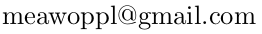
\includegraphics[scale=1.5]{email-address.png} \\ \href{https://meawoppl.github.io/portfolio}{Art Portfolio}  \\ Signal: mattyg.01}

\address{{\bf Work} \\ 2051 Harrison St. \\ San Francisco, CA 94110 \\ (415) 234-3549 \\ \href{https://meawoppl.github.io/resume/MatthewGoodman.pdf}{This Resume}}

\begin{resume}

\section{Objective}
\textbf{I want to build the tools that take electrons to bits, bits to hardware, hardware to firmware, 
firmware to software, software to systems, and systems to positive human impact.}

\section{Work Experience and Leadership}

{\bf CEO \& Founder,} \href{http://www.exclosure.io}{Exclosure} \hfill
Nov 2021 -- Jan 2025
\begin{itemize}  \itemsep -2pt
  \item Founded company, raised $\sim$ 2mm in venture capital, recruited early team.
  \item Created worldwide space monitoring network of $\sim$ 30
        in-house manufactured custom optical telescopes with round the clock global operation.
  \item Designed and manged \textbf{custom AI/ML models} for space object tracking and identification.
  \item Bid and won FFP contracts with NOAA/DOC for commercial space tracking pilot.
  \item Accepted into TAP Lab and Catalyst accelerator programs funded by US SpaceForce.
  \item Proposed, won, and executed AFWERX STTR project.
  \item Led development of electrical, mechanical design, and software stack.
  \item Integrated against existing space tracking networks, and developed custom
        software for data analysis and visualization.
\end{itemize}

{\bf Technical Mercenary,} Various \hfill
\begin{itemize}  \itemsep -2pt
  \item \href{https://www.genrad.com/}{General Radar} -- Developed and implemented a novel radar control algorithms
        for PARCS defense radar. Worked with a team of engineers to implement/validate from high
        level web UI to low level \textbf{FPGA controls}. (2024/2025)
  \item \href{https://starfishneuroscience.com/}{Starfish Neuroscience} -- Aided in the design, build, and prototype of a transcranial
        focused ultrasound stimulation device. Roles ranged from simulation \& modeling to
        mechanical, electrical, acoustic, integration and testing. Led significant investigation
        of human skull geometry variation investigation across a large population. (2020)
  \item \href{https://endiatx.com/}{Endiatx} -- Implemented, \textbf{in Verilog}, complete image acquisition, compression, and radio
        transmission for ingestible pill robot. Advised electrical design for extremely power limited application.
        Integration testing and EE flex design bring-up and testing. (2019/2020)
  \item \href{https://aom.us/}{Arizona Optical Metrology} -- Build high performance computational optics design software
        for the translation of designs to reified \textbf{VLSI mask artwork}.
        Replaced existing tool with complete back-compatibility, 10,000x speed increase and enhanced accuracy.
        Built OSS GDSII tooling optimized for the JVM ecosystem. (2020/2021)
\end{itemize}

{\bf CTO \& Co--Founder,} \href{http://www.3scan.com}{3Scan} \hfill
May 2011 -- May 2019
\begin{itemize}  \itemsep -2pt
  \item Led data intensive biotech startup from foundation to merger with Strateos
  \item \textbf{Grew the organization through four doublings of staff, from 4 to 80+}
  \item Hired, managed, and developed ICs and leads, totaling $> 100$ engineers across 8 years.
  \item Worked with cofounders, board, VCs, leads, and pharma partners to provide strategic vision,
    technical roadmap, and delivered product
  \item Managed creation of high performance $(\approx 50 \mathrm{Gb/s})$, big-data $(> 10\mathrm{PB})$ \textbf{tooling for
    storage, analysis, and visualization} of 3d histological data
\end{itemize}

{\bf President,}  \href{http://coupdefoud.re}{Coup De Foudre} \hfill   Fall 2015 -- Present
\begin{itemize} \itemsep -2pt
  \item Created and lead a high-voltage technical arts troupe
  \item Delivered Burning Man 2019 Honorarium art project ``Theophany''
  \item Incorporated and maintained a 501c3 charity structure
  \item Curate relationships with donors, museums, and grantees
  \item Portfolio: \href{https://meawoppl.github.io/portfolio.html}{https://meawoppl.github.io/portfolio.html}
\end{itemize}

{\bf Scientific Data Analyst,} \href{https://www.atimetals.com/}{ATI Allvac} \hfill
Summer 2007 -- Summer 2008
\begin{itemize} \itemsep -2pt
  \item Unified huge body of process data from several databases for purposes of ML application
  \item \textbf{Developed ML tools for engineers and analysts} to model casting/forging processes
  \item Automated process simulation of solidification for process control and improvement
  \item Implemented custom data analysis for plant process improvement resulting in large
        cost savings by predictive/preventive maintenance of heavy industrial equipment
\end{itemize}

{\bf Consultant,} PACE Metallography, ATI Allvac, Phoenix Heat Treating \hfill Various

{\bf Graduate Researcher,} \href{https://www.utexas.edu/}{University of Texas at Austin} \hfill
Fall 2010 -- Fall 2012
\begin{itemize} \itemsep -2pt
  \item Computational modeling and imaging analysis of the primary visual cortex of primates
  \item Development of \textbf{novel ML techniques} for medical image based recommendation systems
  \item Literal monkey wrangling
\end{itemize}

{\bf Graduate Research Assistant,} \href{https://www.arizona.edu/}{University of Arizona} \hfill
Fall 2008 -- Spring 2010
\begin{itemize} \itemsep -2pt
  \item Modeled heat and mass transfer for NASA/ESA space solidification experiments on ISS
  \item \textbf{Developed HPC CFD solver} for solidification, microfluidics, and biological systems
  \item Worked with ISS payload operations on-site in Huntsville Alabama 
\end{itemize}

{\bf Project Leader,}  \href{https://seds.arizona.edu/}{SEDS} ``Rockoon''  project \hfill   Fall 2008 -- Spring 2010
\begin{itemize} \itemsep -2pt
  \item Led team of two--dozen undergraduates in interdisciplinary design project
  \item Responsible for FAA Clearances and safety of high-altitude high-power rocketry
\end{itemize}

{\bf President,} \href{https://ceramics.org/members/member-communities/classes/keramos}{Keramos} \& {\bf Vice--President,} Material Advantage \hfill Fall 2007 -- Spring 2008
\begin{itemize} \itemsep -2pt
  \item Provided tutoring, and social organization
  \item Led $\sim$ 10 students in outreach, teaching, and grant-writing.
  \item Keramos Awarded ``Most Improved Chapter'' in 2008
\end{itemize}

{\bf Treasurer -- President,} h+ Tucson \hfill Fall 2007 -- Spring 2008
\begin{itemize} \itemsep -2pt
  \item Organized a technoprogressive journal club
  \item This group became \href{http://hplusmagazine.com/}{\textit{h+ magazine}}
\end{itemize}

{\bf MSE Laboratory TA/Preceptor,} University of Arizona \hfill Fall 2007 -- Spring 2008
\begin{itemize} \itemsep -2pt
  \item MSE 414 -- Solidification of Castings -- Ran aluminum casting laboratory
  \item MSE 223 -- Materials Processing -- Taught three groups of 5--7 about materials processing
  \item MSE 110 -- Solid State Chemistry -- Oversaw MSE related lab activities
\end{itemize}

{\bf Barista,} Starbucks \hfill Fall 2005 -- Fall 2008

\section{Patents \& Publications}

  F\,Aeffner, M\,Zarella, N\,Buchbinder, M\,Bui, \textbf{M\,Goodman}, 
  D\,Hartman, G\,Lujan, M\,Molani, A\,Parwani, K\,Lillard, O\,Turner,
  V\,Vemuri, A\,Yuil-Valdes, and D\,Bowman
  ``Introduction to Digital Image Analysis in Whole-slide Imaging''
  \href{http://www.jpathinformatics.org/temp/JPatholInform1019-318182_000518.pdf}{Digital Pathology Association, 2019.}

  \textbf{M\,Goodman}, T\,Huffman, C\,Daniel
  ``Spatial multiplexing of histological stains''
  \href{https://patents.google.com/patent/US20170011511A1/en}{US Patent App.\,15/205,288}

  C\,Daniel, \textbf{M\,Goodman}, K\,Sean, T\,Huffman
  ``Methods and apparatuses for sectioning and imaging samples''
  \href{https://patents.google.com/patent/US20160290895A1/en}{US Patent App.\,15/084,186}

  S\,Raghavan, \textbf{M\,Goodman}, T\,Huffman, C\,Daniel, C\,Monteith, J\,Kwon
  ``Internet-connected high-throughput and high-resolution three-dimensional tissue scanner to
  enable large-scale automated histology''
  \href{https://doi.org/10.1109/IST.2016.7738254}{Imaging Systems and Techniques (IST), 2016.}

  \textbf{M\,Goodman}, C\,Daniel
  ``Motion strategies for scanning microscope imaging''
  \href{https://patents.google.com/patent/US20150138532A1/en}{US Patent App.\,14/529,503}

  C\,Sung, Y\,Choe, \textbf{M\,Goodman}, T\,Huffman,
  ``Scalable, Incremental Learning for Cell Detection in High-Throughput 3D Microscopy Data''
  \href{https://doi.org/10.1109/IJCNN.2013.6706769}{International Joint Conference on Neural Networks 2013.}

  AG\,Hendrick, RG\,Erdmann, \textbf{MR\,Goodman},
  ``Practical Considerations for Selection of Representative
  Elementary Volumes for Fluid Permeability in Fibrous Porous Media,''
  \href{http://dx.doi.org/10.1007/s11242-012-0051-8}{Transport in Porous Media.\,Volume 94.\,2012.}

  \textbf{MR\,Goodman}
  ``Brain--Machine Interfaces'' -- Chapter 26 of \textit{New Materials and Technologies For Healthcare.}
  \href{http://amzn.com/1848165587}{ISBN: 978-1848165588.} 2012.

  RG\,Erdmann, AG\,Hendrick, and \textbf{MR\,Goodman}
  ``Properties of Stochastic Permeability,''
  \href{http://dx.doi.org/10.1007/s12666-009-0038-5}{Transactions of the Indian Institute of Metals. 2011.}

\section{News \& Publications}
  ``An operating system for the biology lab'' \\
  \href{https://www.nature.com/articles/d41586-019-02875-z}{\textbf{Nature Outlook}} \hfill Sept.\,2019

  ``Three-dimensional Imaging and Scanning: Current and Future Applications for Pathology'' \\
  \href{https://www.ncbi.nlm.nih.gov/pmc/articles/PMC5609355/}{\textbf{Journal of Pathology Informatics}} \hfill Sept.\,2017
  
  ``3Scan raises \$14 million for a robotic microscope that could accelerate drug discovery'' \\
  \href{https://techcrunch.com/2016/07/11/3scan-raises-14-million-for-a-robotic-microscope-that-could-accelerate-drug-discovery/
  }{\textbf{TechCrunch}} \hfill July 2016
  
  ``Digital Imaging On The Cutting Edge Of Tissue Analysis'' \\
  \href{https://www.forbes.com/sites/joshwolfe/2015/01/28/digital-imaging-on-the-cutting-edge-of-tissue-analysis/}{\textbf{Forbes}} \hfill Jan.\,2015
  
  ``Mapping brain circuitry with a light microscope'' \\
  \href{https://www.ncbi.nlm.nih.gov/pmc/articles/PMC3982327/}{\textbf{Nature Methods}} \hfill June\,2013
  
\section{Presentations}
  ``Imaging Satellites for Fun and Profit''
  Space Symposium \hfill April.\,2024

  ``Cloud Pathology''
  [re:Invent] Cloud Computing for Biotech R\&D \hfill Oct.\,2018

  ``New Approaches for Volumetric Pathology.''
  MICCAI COMPAY \href{https://sites.google.com/site/compaysymposium2018/speakers}{2018 Workshop} \hfill Sept.\,2018

  ``Digital Pathology Challenges''
  Vision Industry and Technology Forum \hfill Dec.\,2017

  ``Make Dangerous Art''
  Ignite Talks \hfill Sept.\,2017

  ``The Physics of Tesla Coils and Swing-Sets''
  Ignite Talks \hfill Sept.\,2016

  ``10 Tools for Everything''
  Lightning talk at SciPy \hfill June\,2012

\section{Education}
  PhD.\,Biomedical Engineering (Incomplete) \\
  \href{https://www.bme.utexas.edu/}{University of Texas at Austin}
  
  M.S.\,Materials Science and Engineering,
  (GPA 3.83/4.0) \\
  Thesis: \href{http://hdl.handle.net/10150/193422}{``Properties of Stochastic Flow and Permeability of Random Porous Media''} \\
  \href{https://mse.engineering.arizona.edu/}{University of Arizona}, Tucson, AZ
  
  B.S.\,Materials Science and Engineering (In major GPA 3.55/4.0) \\
  \href{https://mse.engineering.arizona.edu/}{University of Arizona}, Tucson, AZ

% I don't think anyone cares about this any more...
\section{Academic Honors}
UT -- NIH NRSA Fellowship for Imaging Science and Informatics \hfill 2010--2011 \\
UA -- Dean’s List \hfill 2007--2008 \\
UA -- ASM International -- Darko Babic Scholarship \hfill 2007--2008 \\
UA -- College of Engineering -- Award for Academic Distinction \hfill 2005--2008 \\
UA -- College of Engineering -- Departmental Honors for Outstanding Achievement \hfill 2005--2006

\section{Languages and Tools}
 \begin{tabular}{l p{5.5in}}
   \underline{Powerful With:} & English, Python, Java, c, Verilog, AWS/GCP,  Rust+Yew \\
   \underline{Useful with:}   & Ts/Js, Docker, c++, CUDA, \LaTeX, bash \\
   \underline{Shipped:}       & Golang, Kotlin, Electron, React Native, Unity, C\#, Swift, bash x86 ASM \\
   \underline{Used Ever:}     & Japanese, FORTRAN, qBasic, php, sql, RoR, bash, Meteor, MATLAB \\
 \end{tabular}

\section{Miscellaneous}
  \begin{tabular}{l p{5.5in}}
    \underline{OSS Contributions:} & cPython, numba, scipy, pandas, pytest, OpenCV, libcamera, esp-idf, \\
                                   & pycuda, datadog, emscripten, progressbar, mingds, mahotas, bottleneck, \\
                                   & meteor  \\
    \underline{Interests:}         & Brain-Machine Interfaces, Computational Geometry, Rock Climbing, woodworking,\\
                                   & Blacksmithing and Casting, High Power Electronics, EDA Software, \\
                                   & Abstract Algebra, Group-Theory, Quasicrystals, Satellites, Astronomy, \\
                                   & SciFi, Bicycles, Computational Geometry, Timelapse Photography
 \end{tabular}

\end{resume}
\end{document}
